\chapter{Proposta de Distribuição da Aplicação PON}
\label{cap:proposta}

Esta proposta investiga a viabilidade técnica da distribuição de uma aplicação de prova de conceito fundamentada no Paradigma Orientado a Notificações (PON), utilizando uma infraestrutura de contêineres orquestrados pelo Kubernetes.

A arquitetura do PON caracteriza-se pela colaboração entre entidades responsáveis pela representação de fatos e pelo processamento de decisões lógicas. Essas entidades interagem por meio de notificações, permitindo organizar o processamento em componentes com responsabilidades específicas \cite{kossoski2024applsci,kossoski2024tese}. Entretanto, o desacoplamento lógico entre entidades não implica, necessariamente, que possam ser distribuídas individualmente entre processos ou nós computacionais sem adaptações.

A investigação deverá considerar as características da aplicação de prova de conceito, suas dependências e os mecanismos de comunicação entre componentes. A partir dessa análise, pretende-se identificar possibilidades de organização da aplicação em unidades de execução conteinerizadas, considerando os custos de comunicação, o compartilhamento de estado e a preservação do comportamento das notificações.

O Docker será utilizado para empacotar a aplicação e suas dependências \cite{docker2026documentation}, enquanto o Kubernetes será empregado para organizar a implantação e o gerenciamento dos componentes em um cluster \cite{kubernetes2026documentation}. A escolha de recursos como \textit{Deployments}, \textit{Services} e \textit{ConfigMaps} dependerá das necessidades concretas da implementação.

A Figura~\ref{fig:metodoproposto} ilustra uma hipótese arquitetural preliminar, não uma implementação validada. A possibilidade de distribuir individualmente as entidades representadas depende da análise das características da aplicação.

\begin{figure*}[tb]
\centering
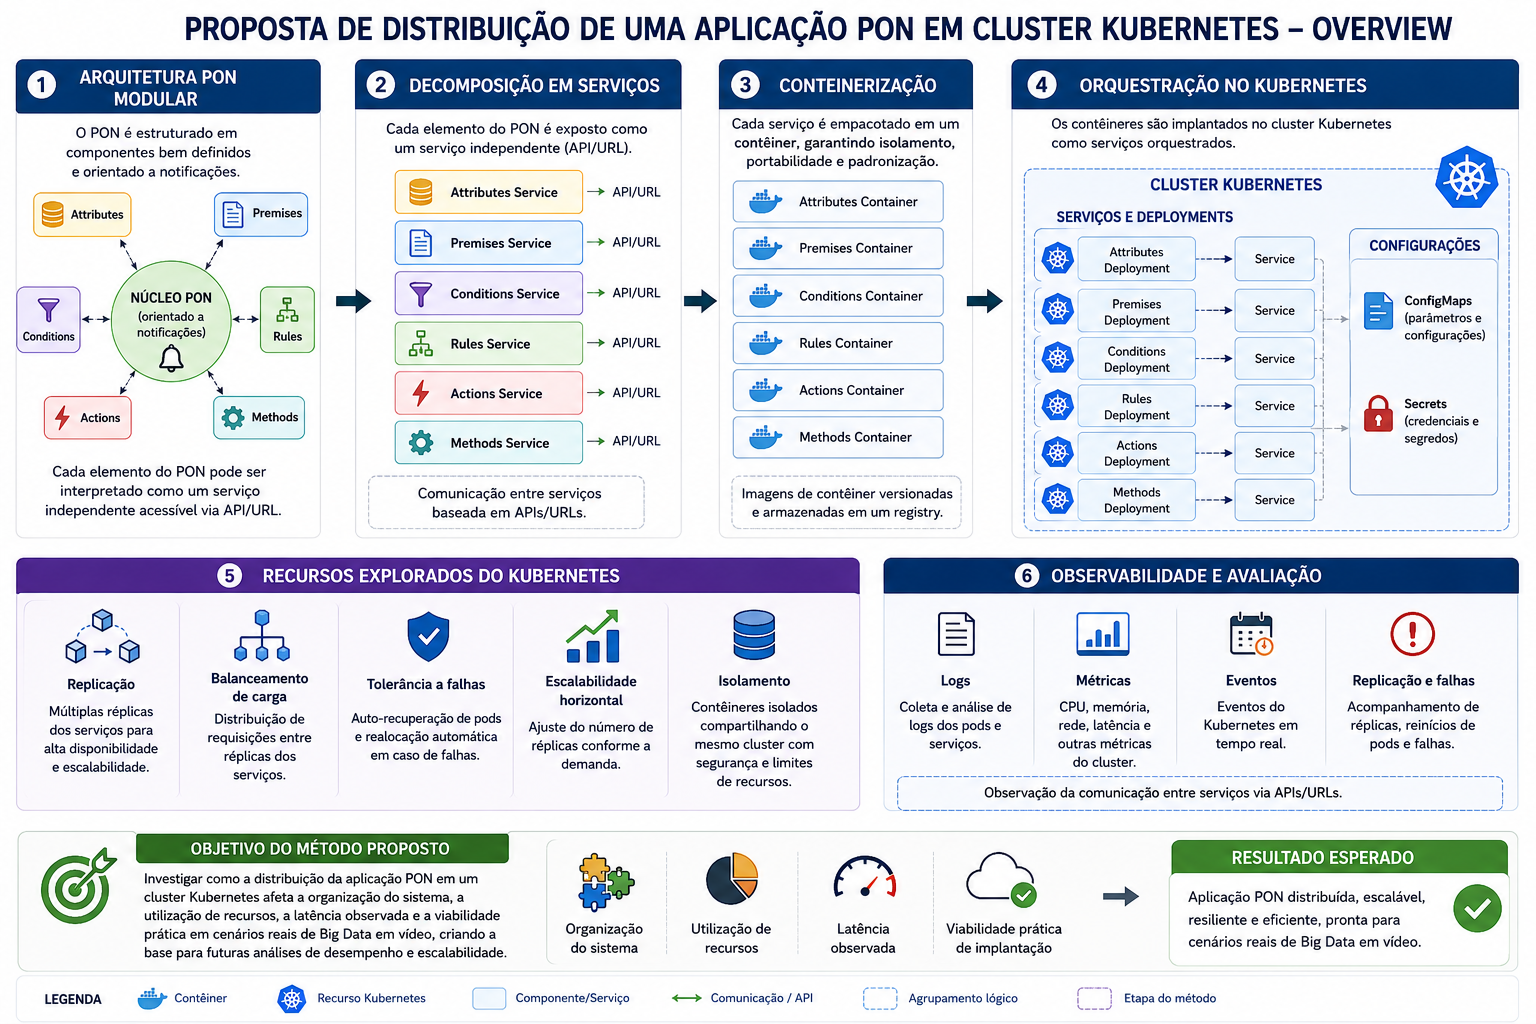
\includegraphics[width=0.99\linewidth]{figuras/proposta-distribuicao-pon-kubernetes.png}
\caption{Hipótese preliminar de distribuição das entidades PON, sujeita a validação técnica.}
\label{fig:metodoproposto}
\end{figure*}

A avaliação deverá considerar o funcionamento da aplicação, a comunicação entre componentes e as dificuldades da implantação. Caso tecnicamente viável, um protocolo experimental poderá incluir consumo de recursos, latência e comportamento sob diferentes configurações. A utilização do Kubernetes, isoladamente, não será considerada evidência de ganhos de desempenho.

\section{Cronograma preliminar}

A Tabela~\ref{tab:cronograma} apresenta um planejamento relativo elaborado no TCC1. Os períodos M1 a M8 ainda não correspondem a meses civis definidos; esse mapeamento deverá ser atualizado após a confirmação do calendário do TCC2.

\begin{table}[htbp]
\centering
\caption{Cronograma preliminar do TCC1 (períodos relativos)}
\label{tab:cronograma}

\small
\renewcommand{\arraystretch}{1.3}

\begin{tabular}{p{7.2cm}cccccccc}
\hline
\textbf{Etapa} &
\textbf{M1} &
\textbf{M2} &
\textbf{M3} &
\textbf{M4} &
\textbf{M5} &
\textbf{M6} &
\textbf{M7} &
\textbf{M8} \\
\hline

Revisão bibliográfica sobre NOP, NOP Query, Docker e Kubernetes
& X & X & & & & & & \\

Estudo da aplicação prova de conceito
& X & X & X & & & & & \\

Preparação do ambiente de desenvolvimento
& & X & X & & & & & \\

Conteinerização da aplicação
& & & X & X & & & & \\

Configuração do cluster Kubernetes
& & & & X & X & & & \\

Implantação e testes iniciais
& & & & & X & X & & \\

Coleta de observações e resultados
& & & & & & X & X & \\

Escrita e revisão do TCC
& X & X & X & X & X & X & X & X \\

\hline
\end{tabular}
\end{table}
